\chapter{Analysis and Design}
This chapter describes all the changes and additions made to Issie by this project, as well as organisational decisions. Additionally, the rationale behind these changes, including analysis of high-level methods, will be explained. 
\section{Approach towards Software Development}
Features were added to Issie using an incremental and Agile approach \cite{Voorhees2020}.
The incremental approach seeks to write code through a repeated cycle of three steps: (1) Analysis and Design, (2) Writing Code, and (3) Testing. A basic task/requirement is  broken into several parts - with each of these parts being written as an individual function \footnote{"individual function" does not refer to a single F\fsharp function, but to a top-level function which uses groups of helper and sub-functions}. Each function is tested both as a unit and when integrated into the codebase. All of these different parts build upon one another and come together to deliver the desired functionality. One caveat of the incremental approach is that the intermediate versions of the app are incomplete and therefore not suitable for any kind of release or proper demonstration. This can make it difficult to get proper feedback on the state of the application as a whole. This was acceptable within short time-frames, but not for long-term software development over the course of the project. For that case, the Agile approach was considered. Small features, represented as a short sequence of stories, were built using the aforementioned incremental approach during sprints. Upon completion of each feature, it could be considered that a new "product" (slightly improved version of Issie) was delivered. During each project meeting, feedback was obtained on the work completed, and any necessary adjustments will spawned new user stories. Agile is generally used in continuous software development projects; however, due to the constraints of a Final Year Project: deadlines, need for planning and report writing, a pure Agile approach was not deemed suitable. Instead, a hybrid approach was pursued, one which embodies Agile principles while still working within a plan-based framework. During the planning phase, the backlog of user stories was intelligently structured such that epics were ordered by importance to the project, and stories within the epics were structured such that features would be added incrementally. This ordered backlog can be found within the work breakdown structure (WBS) described in Figure \ref{fig:wbs2} in Appendix \ref{app:wbs}.
\section{Technology Stack}
This project does not make any deviations from Issie's existing technology stack, described in Section \ref{sec:techstack}. The F\fsharp application code is compiled to JavaScript using the Fable compiler, and is run as a web app in a desktop environment using Electron. The user interface is powered by React and the MVU architecture, brought to the F\fsharp ecosystem by the \codestyle{Fable.React} and \codestyle{Elmish} libraries. New files added to the Issie codebase by this project are split between two existing directories in the \textit{Renderer} project. Files which implement features related to actual truth table generation and reduction are placed in the \textit{Simulator} directory, while files which implement the UI are placed in the \textit{UI} directory. 

% \section{Overview of Added Features}
% This section describes all the changes and additions made to Issie by this project. In subsequent sections in this chapter, the rationale behind these changes, including analysis of high-level methods, will be explained. Finally, in the Implementation chapter, the details of how these features were implemented will be explained. 

\section{Top Level UI Changes}
The top-level UI of the application has been changed to accommodate truth tables. As a result of this, the way the waveform simulator is accessed has been changed as well. In prior versions of Issie, the right tab section had three options: \textbf{Catalogue} for adding new components, \textbf{Properties} for changing component properties, and \textbf{Simulation} for launching the Step Simulator. When applicable, Waveform Simulator could be accessed by clicking a button in the top bar, which would temporarily create an extra tab in the right section. Given that most interactions related to modifying or gaining insight into the schematic were done through the right section tabs, the decision was made for the truth table to be displayed there. The large amount of space needed to display a truth tables and related functionality warranted a separate tab for truth tables. However, this approach posed some potential problems. During the earlier evaluation of Issie, it was found that the method of accessing the waveform simulator was inconsistent, and that the waveform simulator should ideally have it's own permanent tab too. Therefore, the total number of tabs would increase from three to five, resulting in a cramped layout. 
The updated version of Issie delivered by this project solved this problem by grouping all circuit simulation activity under one tab. The third tab in the right section has been re-named to \textbf{Simulations} and features three further sub-tabs, each for the Step Simulator, Truth Table generator, and Waveform Simulator respectively. This can be seen in Figure \ref{fig:issieview}, where the \textbf{Truth Table} sub-tab is open. 
From this tab, the user can choose to generate a truth table for the whole sheet. Additionally, if a correct configuration of components is selected, a second option to generate a truth table for the selected configuration is also shown to the user. As with the Waveform Simulator, when the Truth Table tab is open, the dividerbar can be dragged to resize the right section. Previously, there was a bug where, if the right section was scrollable, the dividerbar height did not dynamically resize. This bug was fixed by this project.
\begin{figure}[h]
    \centering
    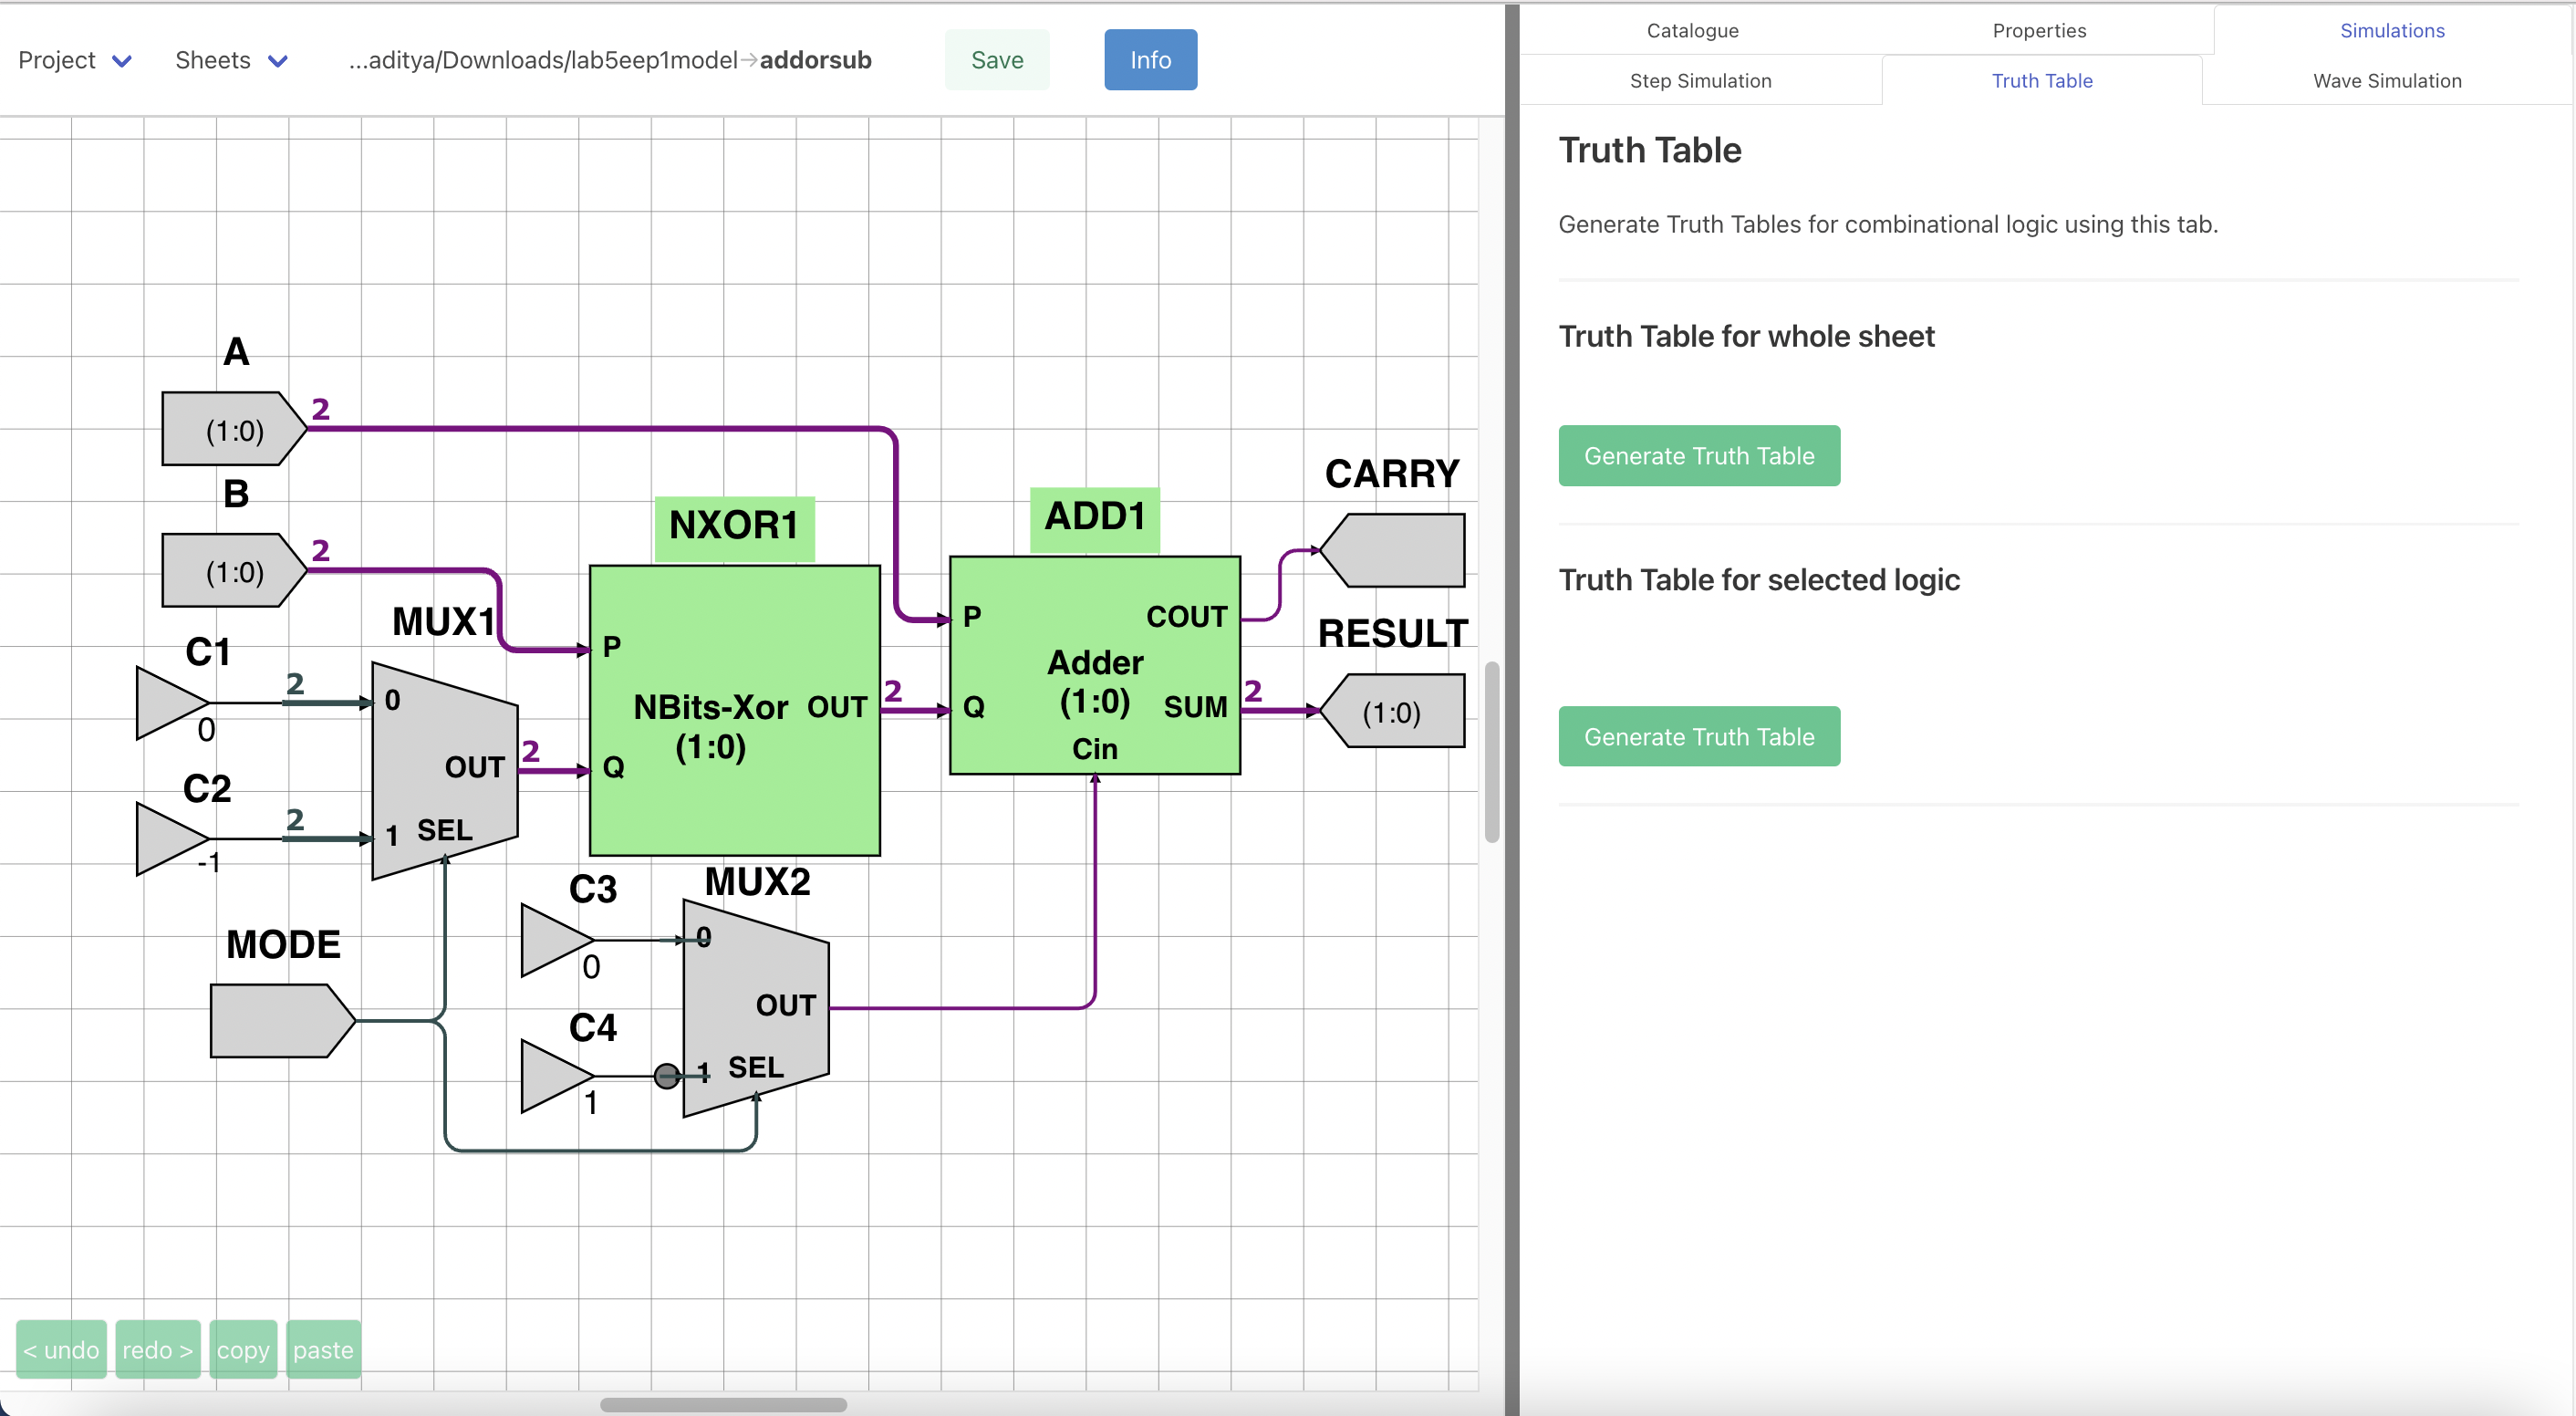
\includegraphics[width=\textwidth]{04.AnalysisDesign/Issieview.png}
    \caption{View of Issie's updated Top-Level UI}
    \label{fig:issieview}
\end{figure}

\section{Generating Numeric Truth Tables} \label{sec:analysis_ttGen}
The user can generate a truth table by clicking on the \textit{Generate Truth Table} button. Like the  \textit{Star Simulation} button in the Step Simulator, this button provides feedback on the correctness of the canvas to the user through colours. A green button indicates a correct canvas which can be used to generate a truth table. If there are issues with the schematic, the button will instead be yellow, and clicking it will inform the user of the nature of the error via an error message and highlighting the erroneous component. Finally, the button can also be a faded green; this indicates that while the schematic is correct, it is unsuitable for truth table generation as it contains sequential logic. This is done to maintain consistency with the Waveform Simulator button, which becomes faded when there are no sequential components.

When the user generates a truth table, a numeric truth table is generated at first. Due to performance reasons, which will be discussed later, Issie will only generate up to the first 1024 rows in a truth table. In cases where the truth table should have been larger than this limit, it is considered \textit{truncated}. The user is warned of this through a yellow coloured popup with the following message: \textit{"The Truth Table has been truncated to 1024 input combinations. Not all rows may be shown. Please use more restrictive input constraints to avoid truncation"}. Once a truth table is generated, the user can interact with it in numerous ways through the user interface, transforming and regenerating it as necessary. Figure \ref{fig:tttab} shows two views of the Truth Table tab, which contains a menu with collapsible sections. The compact view (Figure \ref{fig:compact}) is the default, with all sections other than the one displaying the truth table, reduction operations, and base selector being collapsed. The other sections can be expanded to reveal additional functionality; Figure \ref{fig:expand} shows the view of the Truth Table tab when all sections are expanded. The tab section is also scrollable.

Figure \ref{fig:ttGen} shows a high-level overview of the truth table generation process. This process will be covered in more detail in the Implementation chapter, but the overall process can be summarised into three phases: building the simulation, finding the input combinations which make up the left-hand side of the the truth table (Input Space), and simulating each combination in the input space to build the truth table. Decisions had to be made on how to generate the input space, as well as how to simulate each input combination.

\begin{figure}[h]
     \centering
     \begin{subfigure}[b]{0.48\textwidth}
         \centering
         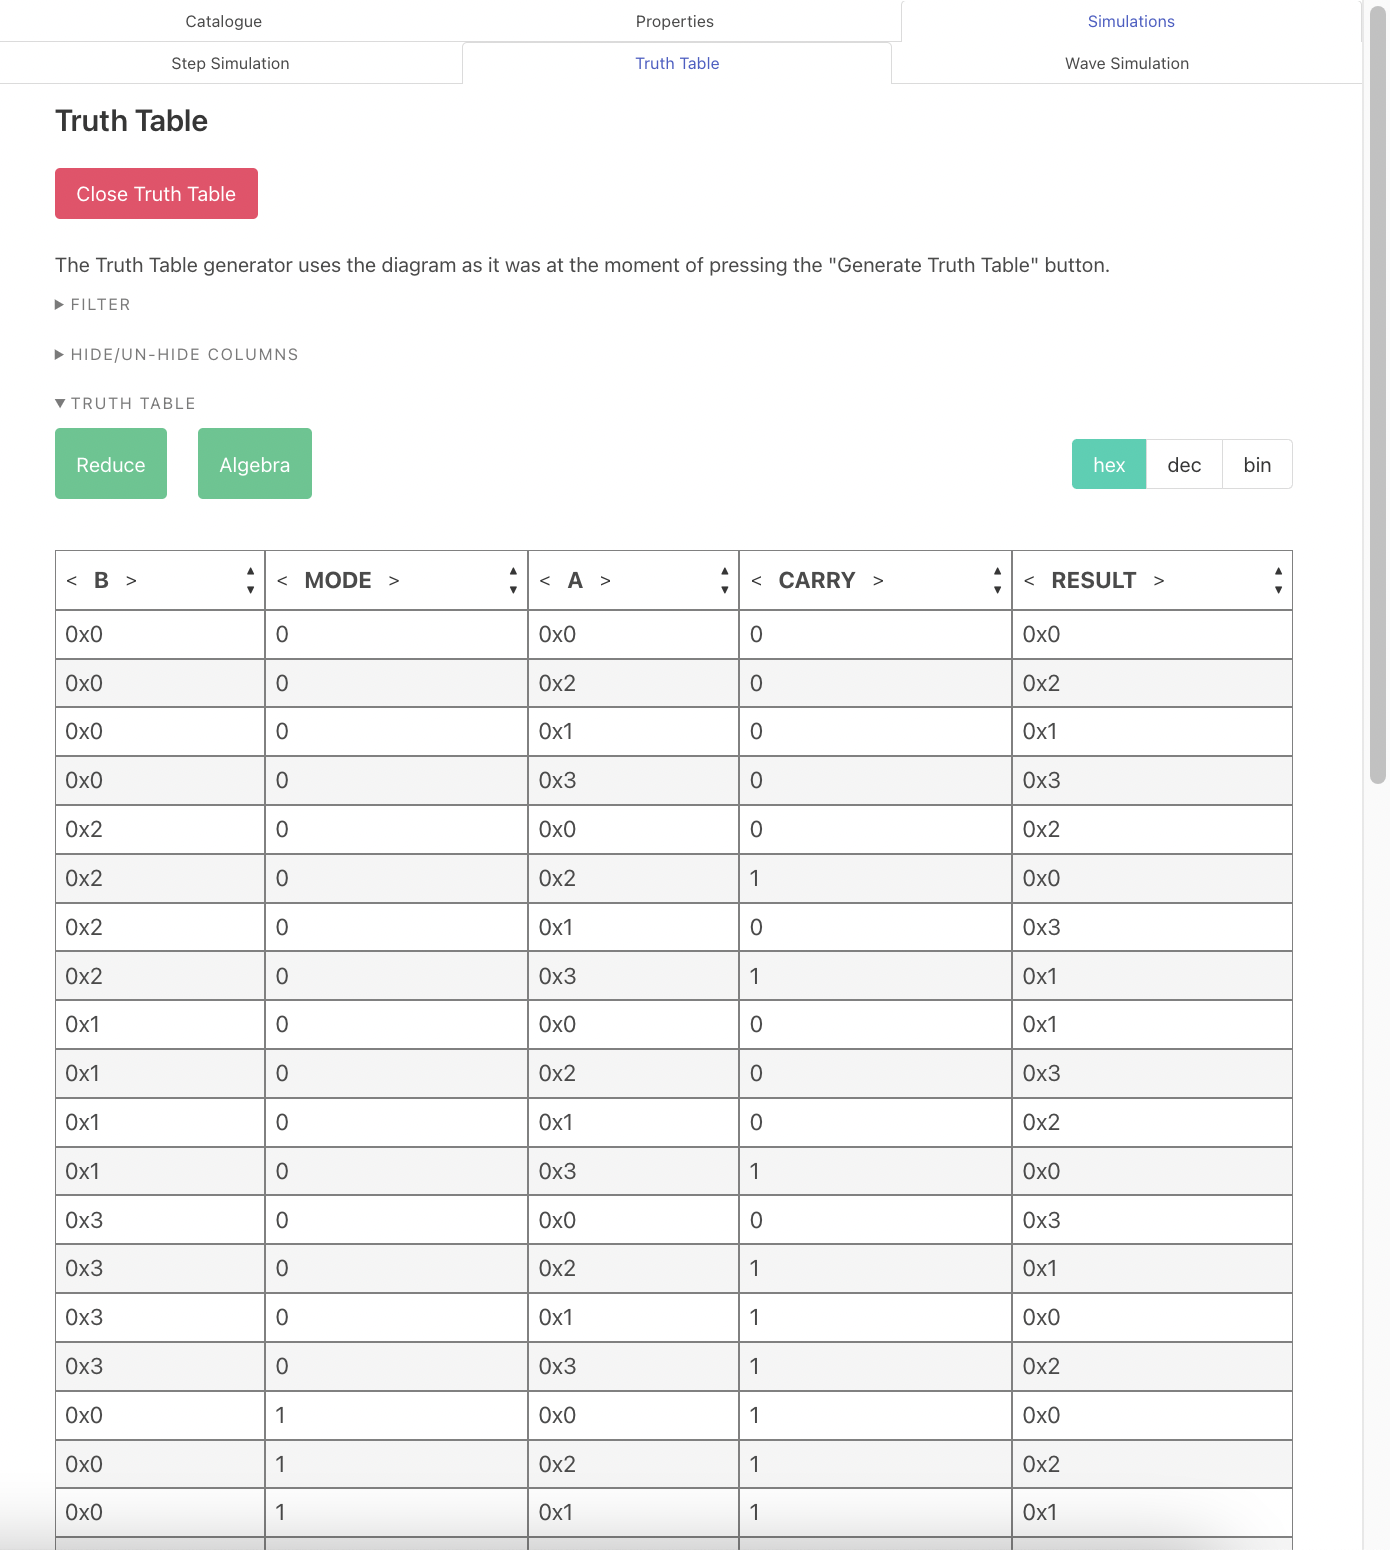
\includegraphics[width=\textwidth]{04.AnalysisDesign/compact.png}
         \caption{Compact View}
         \label{fig:compact}
     \end{subfigure}
     \begin{subfigure}[b]{0.48\textwidth}
         \centering
         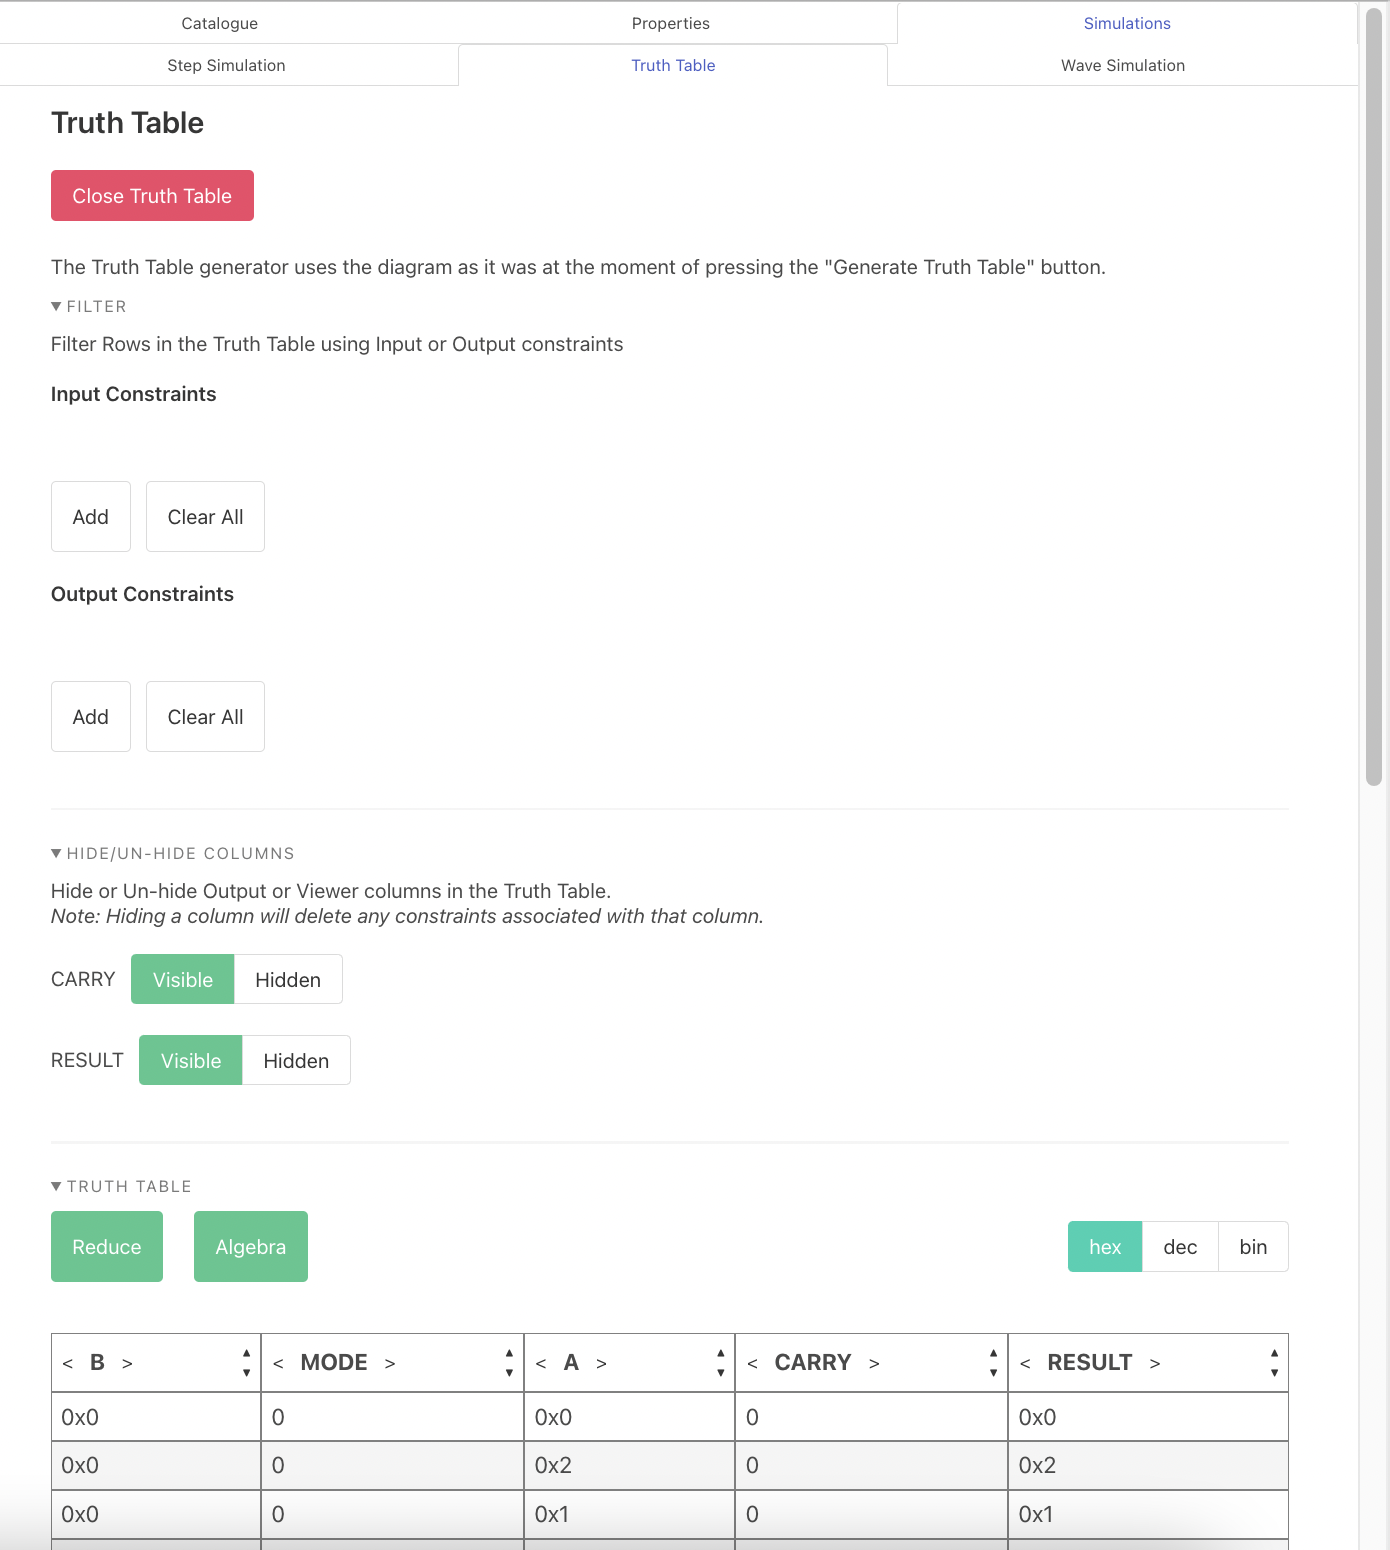
\includegraphics[width=\textwidth]{04.AnalysisDesign/expanded.png}
         \caption{Expanded View}
         \label{fig:expand}
     \end{subfigure}
        \caption{Contents of Truth Table tab after a truth table has been generated}
        \label{fig:tttab}
\end{figure}

A decision also had to be made regarding the handling of multi-bit IOs.
In Issie, inputs to combinational logic can be multi-bit (width > 1), and propagate through the logic via multi-bit buses. Two possible approaches for handling these multi-bit inputs were considered. The first option was to split a multi-bit input into its constituent bits in the truth table; this aligns more closely with the actual hardware implementation of the logic \cite{muxtables}, where component ports only accept a single-bit signal. However, this is not user-friendly at all - for example a 32 bit bus would be split into 32 different inputs. This would massively increase the number of columns in the truth table, impacting the utility of the truth table as an aid. Furthermore, splitting inputs and outputs into separate bits would obscure certain relationships, such as those of arithmetic circuits. Instead, the decision was made to represent each multi-bit input/output as one column in the truth table, with the value shown in hexadecimal format by default. The user can choose between hexadecimal, decimal, and binary representations.

\subsection{Decision to re-use Step Simulation Code}
At its core, generating a complete numeric truth table is a brute-force process. Each possible combination of input values must be simulated to calculate the corresponding output values, and the relationship should be recorded in the table. 
Given that Issie already features a performant and reliable simulator (step simulator) for calculating the outputs of combinational logic, the decision was made to use as much of its implementation as possible. This approach has many advantages:
\begin{itemize}
    \item The existing step simulator has been extensively tested by end-users, meaning that its implementation is most likely bug-free. By using it, it will reduce the chance of the new feature introducing new bugs.
    \item In most cases, reusing existing code is much faster than writing new code from scratch. Not only is time saved on writing new code, but the amount of time spent debugging is also reduced.
    \item Reusing existing code will help keep the overall size of the codebase small. Not only does this help future programmers who work on the project by reducing how much they have to understand, but it also means that any future improvements made to the simulation code are also improvements to Truth Table generation.
\end{itemize}

% Figure \ref{fig:flowchartSim} provides an overview of Issie's process for building and running a Step Simulation. In this process, various checks must be performed; firstly the logic designed by the user must be verified to be syntactically correct, secondly the organisation of project files must be correct, and thirdly some Issie specific limitations (e.g. no cycles in combinational logic) must be enforced. Issie's simulation building process can be said to have three levels, with each level having an associated data structure which represents schematic. These data structures are: the \textbf{Canvas State}, \textbf{Simulation Data/Error}, and a \textbf{Fast Simulation}. A set of checks are performed at each level, and only upon passing these checks can a schematic be transformed to the subsequent data structure.
% If any of these checks fail due to an issue with the user's schematic, the simulation building process returns a \textit{SimulationError}, which tells the user what the error is and which components/connections are affected. A key takeaway from Figure \ref{fig:flowchartSim} is that the process of building a simulation is separate to the process of running it. During the \codestyle{FastSimulation} building process, the schematic is analysed, with components being placed into an appropriate order for combinational reduction. However, as the \codestyle{FastSimulation} data structure is mutable, the values of each input can be updated without having to rebuild the whole simulation. Therefore, the time taken simulating a different input combination is quite short, as only the reduction function has to be re-run to find the new outputs. 
% This distinction between building a simulation and running it with different input values makes the existing Step Simulator an optimal choice for use in truth table generation, which will need to simulate multiple input combinations as fast as possible. 




\begin{figure}[h]
    \centering
    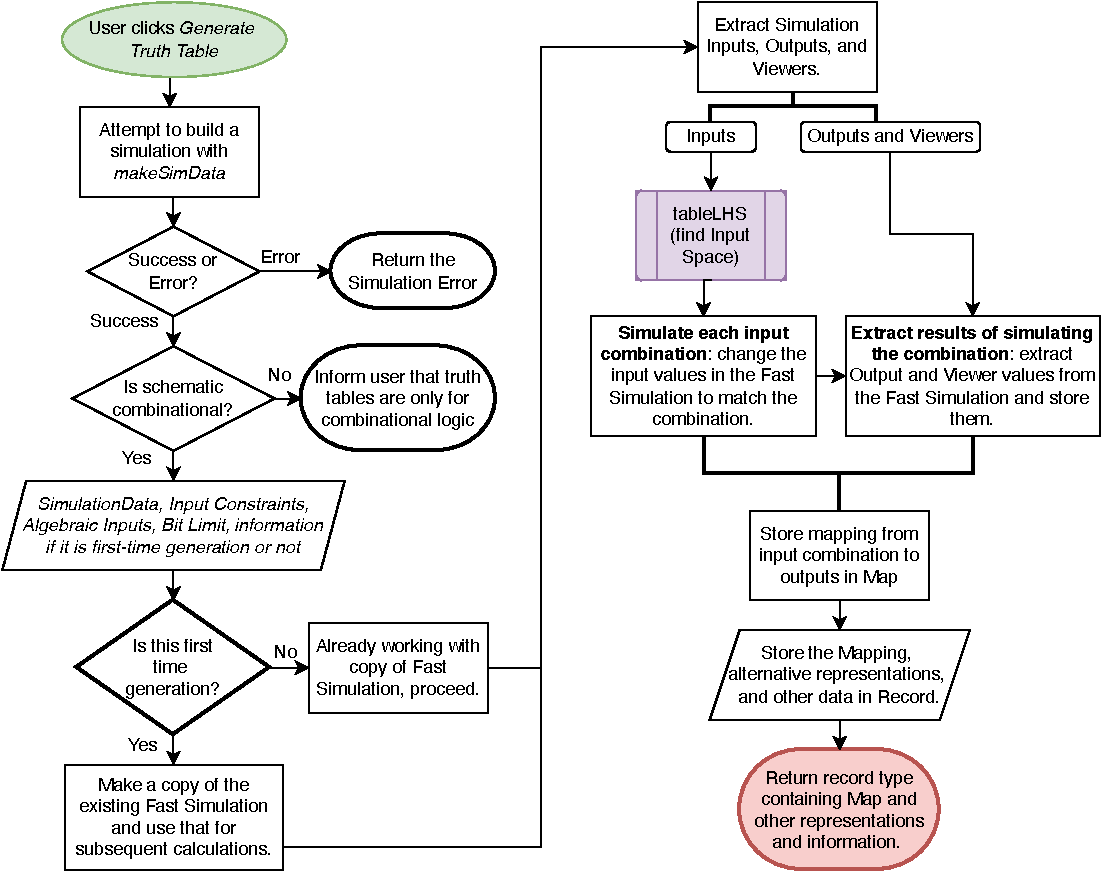
\includegraphics[width=0.8\textwidth]{04.AnalysisDesign/ttGen.pdf}
    \caption{High-Level view of Truth Table Generation}
    \label{fig:ttGen}
\end{figure}

% \begin{figure}[h]
%     \centering
%     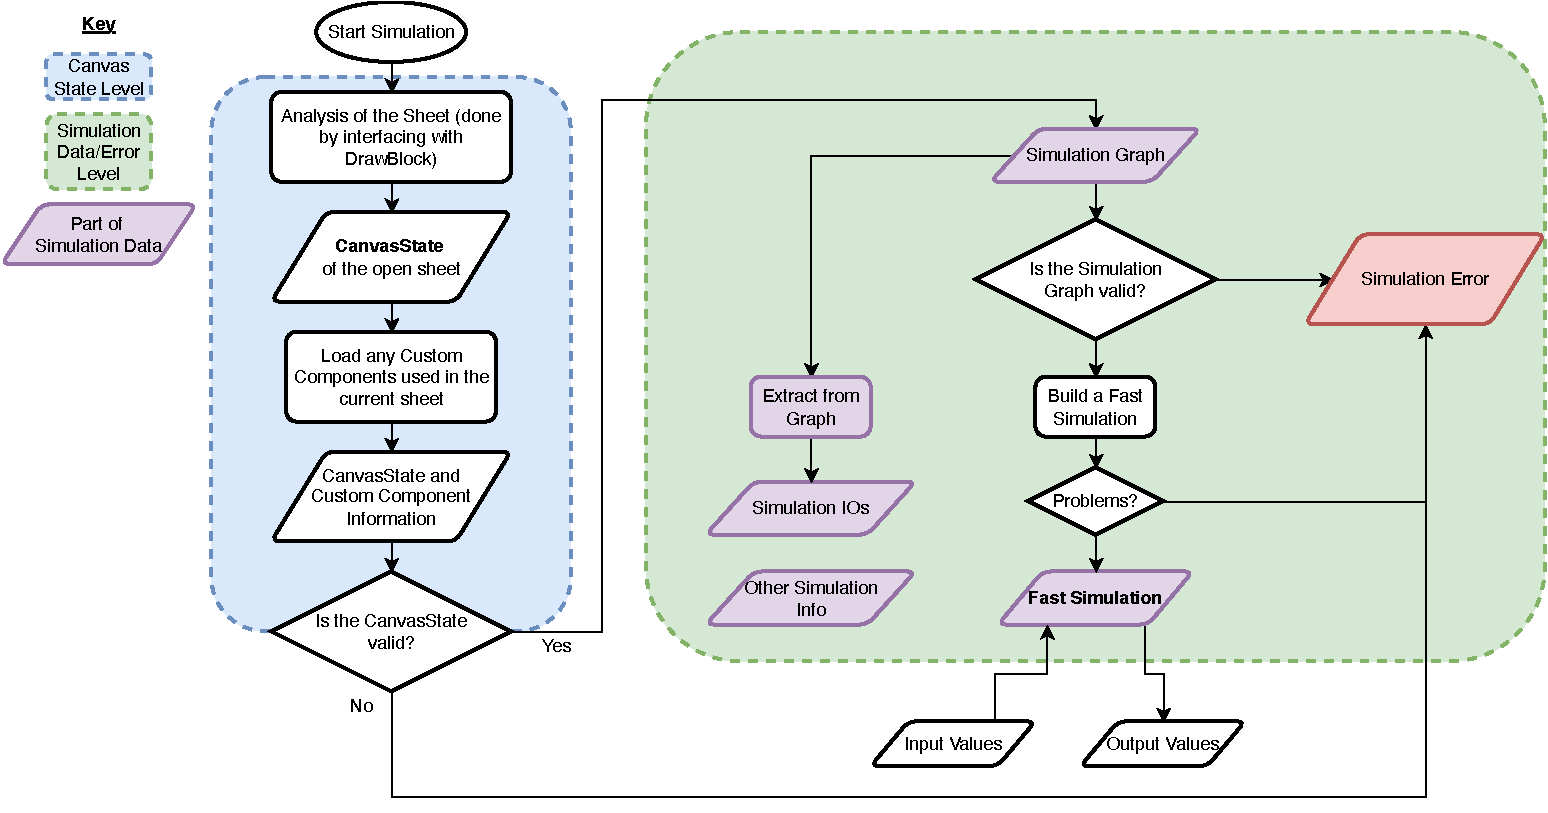
\includegraphics[width=\textwidth]{04.AnalysisDesign/IssieSim.pdf}
%     \caption{An overview of Issie's Step Simulation}
%     \label{fig:flowchartSim}
% \end{figure}

\subsection{Evolution of the Input Space Generation Algorithm} \label{subsec:evolutionofinputspace}
The process of calculating the input space, highlighted in purple in Figure \ref{fig:ttGen}, had two versions. The change from the first to the second version affected the overall structuring of operations on truth tables in the application. Initially, the entire input space was calculated and simulated. This would result in a very large, exhaustive truth table -- one which contained every possible input and output combination. The user would haven been able to reduce this truth table by filtering the table or using Don't Care Reduction. However, several issues arose with this approach, with the most crucial being that of performance. 

For a truth table with $n$ inputs ($x_1 .. x_n$), each of width $w$, ($w_1 .. w_n$), the number of rows in the truth table is given by the sum of all widths raised to the power of 2, as shown in Equation \ref{equ:rowcount}. For example, a schematic with three inputs, with widths: $w_1 = 1, w_2 = 2, w_3 = 3$ would result in a truth table with 64 rows. This sum-of-widths formula is derived from the idea that if we define a set $S_i$ as the set of all possible input combinations for input $x_i$, the left-hand side of a truth table is the \textbf{Cartesian Product} of all sets from $S_1$ to $S_n$. This project defines the left-hand side of the truth table as the \textbf{input space} of the truth table, and the right-hand side as the corresponding \textbf{output space}.
\begin{equation} \label{equ:rowcount}
    \textrm{Row Count} = \prod_{i=1}^{n} 2^{w_i} = \prod_{i=1}^{n} S_i = 2^ {\left( \sum_{i=1}^{n} w_i \right)}
\end{equation}

The complexity of finding the Cartesian product of multiple sets is an exponential function of the number of sets. For example, the complexity of finding the Cartesian product of $n$ sets, each of size $s$, would be $O(s^n)$. The size of each set is dependent on the width of the input; Issie does not limit input widths, meaning that the size of the sets may also be very large. For example, a single 16-bit input has 65536 unique values, and combining this with a second 16-bit input yields an input space of $2^{32}$ combinations (over 4 billion). Simulating this large number of combinations and storing the result takes upwards of 20 seconds, violating essential requirement \textbf{E1.7}. Additionally, a sufficiently large input space could cause the system to run out of memory and crash, which is unacceptable. Along with the practical issues with the generation of the complete truth table, it can also be argued that a very large complete truth table is not useful to the user. According to the Atkinson-Shiffrin memory model described in Section \ref{subsec:memmodels}, external stimuli only stay in the sensory register for 0.5 seconds prior to decaying. A large number of rows is likely to overload the sensory register, meaning that it is likely that the information will not pass to short term memory unless the the user slows down and processes each row one-by-one. Even if this were the case, a truth table with a large number of rows would take over 30 seconds for the user to read and process. Given that short term memory decays in 30 seconds, this means that the user will likely have forgotten the first row by the time they finish reading the last one. Therefore, the method of generating and simulating the entire input space to create an exhaustive truth table was deemed unfit.

As a result, the decision was made to \textbf{truncate the truth table}; generate and simulate only part of the input space. The current limit is 1024 rows. Considering that users would only be able to focus on a small subset of rows at a time, and would likely reduce the size of the table anyways, this approach would sacrifice very little for a significant gain. However, any subsequent operations, such as filtering and reduction, would take place on the truncated table, which does not contain all of the necessary data. The nature of these issues, as well as the steps taken to mitigate them are:

\begin{itemize}
    \item[] \textbf{Issue 1}: Input constraints will be applied to the truncated table, so user may not see a full representation of the relationships for the case they enter. For example, consider the input $X$ which has a width of 8 bits (so values range from 0 to 255), but due to truncation, only rows with values of $X$ up to 31 are present. If the user applies the input constraint $X = 32$ to the table, an empty table will be returned as no rows which fulfil this condition exist in the truncated table.
    \item[] \textbf{Solution 1}: Apply input constraints during truth table generation. This is achieved by using the constraints to determine a tighter input space, and then simulating that. Giving users a way to choose which inputs contribute more to the input space (they can fix certain inputs and let others vary within bounds) allows them to interactively generate truth tables that deliver the most information to them.
    \item [] \textbf{Issue 2}: Output constraints will be applied to the truncated table, which is missing many rows. Due to this, the result of applying the output constraints will include all rows which match the condition.
    \item [] \textbf{Solution 2}: Unfortunately there is not much that can be done to combat this issue alone other than warn the user that they are looking at incomplete results. However, if the user is able to use input constraints to sufficiently reduce the input space first, output constraints could help filter the table further.
    \item [] \textbf{Issue 3}: Don't Care Reduction will occur on the truncated table, which does not fully represent the logical function performed by the circuit. This could result in incorrect relationships being inferred by the reduction algorithm.
    \item [] \textbf{Solution 3} Much like with output constraints, there is no perfect solution as relationships for reduction are inferred from the truth table. Don't Care reduction is therefore limited to smaller schematics which do not produce truncated truth tables. The user is instead guided towards reducing truth tables for larger schematics with \textbf{Algebraic Reduction}.
\end{itemize}

Implementing Solution 1 required a new method of generating the input space. The new method needed to know which sub-sets of the input space it could and could not generate before it actually generated it using the Cartesian product method. Further details of the workings and implementation of this method can be found in the Implementation chapter.

\section{Generating Truth Tables for a partial selections}
The motivation behind Requirement \textbf{E1.2} is that a large schematic with lots of components will often contain smaller blocks of logic within it. These blocks may be defined Custom Components, or simply be a collection of gates in one corner of the canvas. Either way, there is value in the user being able to isolate these blocks and learn about the combinational logic implemented by them. Such functionality would also allow users to take a divide-and-conquer approach to debugging logical errors - individual blocks could be inspected to ascertain if they had been implemented correctly. 

A challenge with generating a truth table from part of a canvas is that Issie has no existing method for simulating part of a canvas. When working with a whole sheet, the inputs and outputs are well-defined; sheets where any ports aren't connected to inputs/outputs throw \textit{Simulation Errors}. In contrast, a partial selection from a sheet will rarely contain all inputs and outputs. Two methods were considered for simulating the selected logic to generate a truth table, with the latter being chosen.
\begin{enumerate}
    \item \textbf{Extracting the Fast Simulation and feeding values into specific wires}. This method would have involved creating a Fast Simulation for the whole sheet as usual, but then manually changing values in component arrays and seeing how those changes propagated through to the output connections of the selected logic. While this method seemed fit initially, several issues were found after some analysis. The Fast Simulation would be built for the whole sheet, meaning that an error elsewhere on the canvas would stop the selected logic from being simulated. Custom Components would also be harder to manage as the Fast Simulation datatype flattens the design, meaning that all nested logic in Custom Components would be expanded out. The new logic would also be quite different from the truth table generation logic for whole sheets - this is not ideal for future code maintenance purposes.
    \item \textbf{Intelligently building and correcting a new Canvas}. Following the highlighting of the issues with the first approach, an alternative approach was put forward. Rather than attempting to work with the complicated Fast Simulation data structure, it instead aims to use as much of the existing code as possible by treating the selected logic as a separate instance of a Canvas State and trying to simulate it using the same method as simulating a whole canvas. The main difference between simulating a whole sheet and simulating selected logic is the lack of guaranteed input and output components. This is overcome by finding which ports/connections are inputs/outputs for the selected logic, then intelligently adding 'phantom' input/output components to the canvas in a process called Canvas Correction. Once a corrected canvas corresponding to the selected logic is created, the logic used for generating and viewing a Truth Table for a whole sheet can be reused.
\end{enumerate}

The method implemented by this project first sanity-checks the part of the sheet the user has selected. Following this, the canvas correction algorithm adds new Input and Output components to the partial selection to transform it into a valid Issie schematic. The existing truth table generation process can then continue using this valid schematic.

\section{Filtering with Constraints}
Once a truth table has been generated, it can be filtered using constraints; these can be equality or inequality constraints. Equality constraints on an input or output (IO) are of the form $IO = value$, where the truth table is filtered such that only rows where the input or output (IO) is equal to the given value are shown. Inequality constraints are of the form $LowerBound \leq IO \leq UpperBound$; the filtered truth table will only contain rows where the IO is between the lower and upper bounds (inclusive). Due to reasons that will be discussed further in this chapter, applying input constraints will re-generate the table, while output constraints will only filter the existing table. 
Constraints are added through a popup window as shown in Figure \ref{fig:addconstraint}. Issie validates all constraints in real time; the user is prevented from entering an invalid constraint and is told the why it is invalid. This can be seen at the bottom of Figure \ref{fig:addconstraint}, where the message informs the user of the issue with the constraint they are trying to add. This approach has two major advantages. Firstly, from a system design perspective, the logic which applies the constraints can trust that all the constraints are well-formed and do not conflict with one another, maintaining robustness. Therefore error handling for constraints need not be implemented in these sections. Secondly, from a user experience perspective, this approach is more obvious and intuitive, aligning it with Issie's core principles. The issue with the user input (invalidity of the constraint) is addressed at the moment it happens, making it clear to the user exactly what has gone wrong. This is far more clear than propagating the error to the user later on in the process.
Once added, the constraint will appear as a small tag in the Filter section -- the constraint can be deleted by clicking the cross on the tag; alternatively all input or output constraints can be cleared by clicking the \textit{Clear All} button for each respective group.
\subsection{Constraint Validation Rules}
\begin{enumerate}
    \item All entered values must be valid numbers -- numbers can be entered in decimal, hex (\codestyle{0x}), or binary (\codestyle{0b}) form.
    \item All entered values must not exceed the width of the IO, with checks also implemented for negative numbers (e.g. cannot enter 9 or -6 for a 3-bit IO).
    \item Constraints must be unique; the entered constraint must not already exist.
    \item Constraints must not overlap. For example, if a constraint $X=5$ exists, the constraint $4 \leq X \leq 7$ cannot be added (and vice versa).
    \item For inequality constraints, the upper bound must be greater than the lower bound. This check is always performed using the unsigned representation of the number entered.
\end{enumerate}

\begin{figure}[h]
     \centering
     \begin{subfigure}[b]{0.4\textwidth}
         \centering
         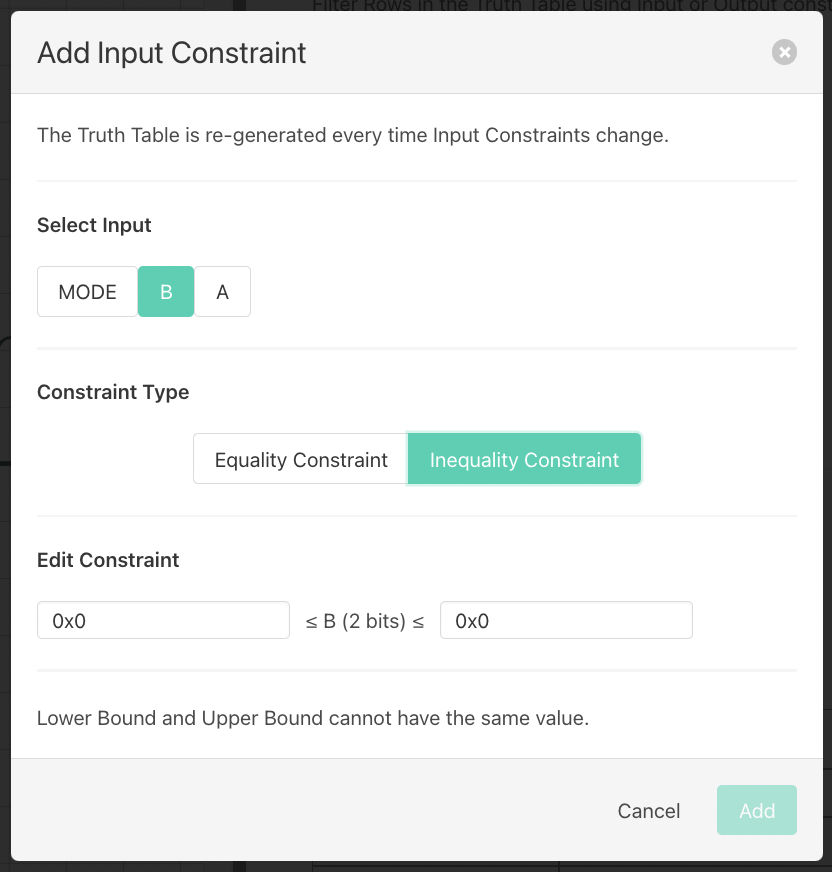
\includegraphics[width=\textwidth]{04.AnalysisDesign/constraintadder.png}
         \caption{Popup for Adding an Input Constraint}
         \label{fig:addconstraint}
     \end{subfigure}
     \begin{subfigure}[b]{0.4\textwidth}
         \centering
         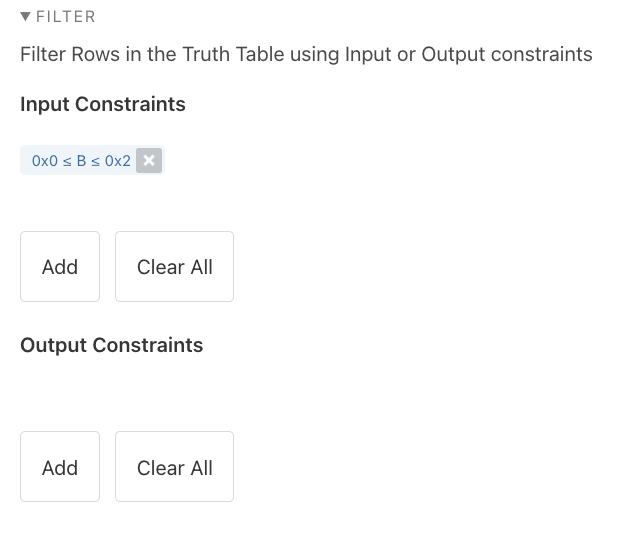
\includegraphics[width=\textwidth]{04.AnalysisDesign/tabwithconstraint.png}
         \caption{Filter section after adding a constraint}
         \label{fig:tabwithconstraint}
     \end{subfigure}
        \caption{Adding a Constraint to the Truth Table}
        \label{fig:constraintadd}
\end{figure}

\section{Hiding Output Columns}
The second menu section allows the user to hide (or un-hide) output or viewer columns from the truth table. This means that the user can choose to focus on relationship between the inputs and a specific output. This may be useful when analysing arithmetic circuits -- the user may wish to hide the carry-out column to only focus on the result. As can be seen in Figure \ref{fig:expand}, each output/viewer has a toggle component which has two options: visible and hidden. These are used to set the visibility of columns in the truth table. The action of hiding at output column takes less than 100ms -- this is classed as instantaneous. Achieving this required specific decisions to be made regarding how to the truth table was rendered; these will be discussed in Section \ref{sec:ttView}.

\section{Graphical Manipulation of Truth Tables}
\textbf{Re-ordering Columns} On either side of each IO label in the heading row, there are left and right arrows. These allow the user to arrange the truth table as they please by changing the order of columns in the truth table.

\textbf{Sorting} In each IO heading cell, there are a pair of up/down arrows for sorting the truth table by the values of that IO. Selecting the up arrow sorts in ascending order, while selecting the down arrow sorts in descending order. Once selected, an arrow remains highlighted (until another is selected), to inform the user of how the truth table is being sorted. The rationale behind implementing truth table sorting is that it allows users to organise the information they view, increasing the control they have over their learning experience. 

\textbf{Auto-resize with dividerbar} The draggable dividerbar can be used to resize the right section. The truth table will dynamically resize to match the set right section width, and contents of cells will wrap to the next line and automatically adjust such that no content is cut off.

All of the operations above happen instantaneously (<100ms); achieving such performance with column-based operations relied on the same decisions as those which made hiding columns appear instantaneous (see Section \ref{sec:ttView}).

\section{Don't Care Reduction} \label{sec:dcreductionanalysis}
If the generated numeric truth table is \textbf{not truncated}, then the user can reduce it through Don't Care reduction. When the user presses the \textit{Reduce} button, the truth table will be analysed, and any rows where certain inputs are redundant will be collapsed, with the value for that input being replaced by an \textbf{X}. The user can always return to the full table by clicking the \textit{Back to Full Table} button. Like their full numeric counterparts, reduced truth tables can also be filtered and sorted.
If the truth table is truncated, Don't Care reduction is unavailable; this is communicated to the user by a greyed-out \textit{Reduce} button. Hovering over the disabled button will show the user a popup explaining why the option is unavailable.

As discussed in Section \ref{subsec:dcbackground}, two possible methods of implementing DC Reduction were considered; either porting an existing heuristic-based minimisation tool to Issie, or writing a reduction algorithm from scratch. Ultimately, the latter was chosen. This is because existing minimisation tools are tailored towards hardware design in industry, where the priority is simplifying the design so it requires fewer components. There is a risk that complicated simplification may in fact obscure the logic further; this is the opposite of this project's intention. Further to this, current minimisation tools like Espresso \cite{espresso} do not support multi-bit inputs and outputs, which would make integration with Issie's existing framework difficult. Given the decision to not split up multi-bit IOs in Issie, Espresso was deemed unfit. The custom reduction algorithm takes an un-truncated numeric truth table and attempts to reduce it by recursively finding redundancies through row comparisons.

\section{Algebraic Truth Tables}
In addition to numeric truth tables, this project also adds algebraic truth tables to Issie. Instead of numerical values, outputs are instead represented as an algebraic function of their inputs. These algebraic functions are loosely based on Boolean algebra, but do include other operators such as addition and subtraction in order to provide a more useful summary of relationships. Users can introduce algebra into an existing numeric truth table by clicking the \textit{Algebra} button above the truth table. This will spawn a popup, where the user can choose which inputs to set as algebraic, and which inputs should remain numerical. There exist cases when certain inputs cannot be set as algebra, such as when an input is connected to the select (SEL) port of a multiplexer. The user is prevented from setting those inputs as algebraic values, and a helpful error message informs the user why. An example of this can be seen in Figure \ref{fig:algpopup}

\begin{figure}
    \centering
    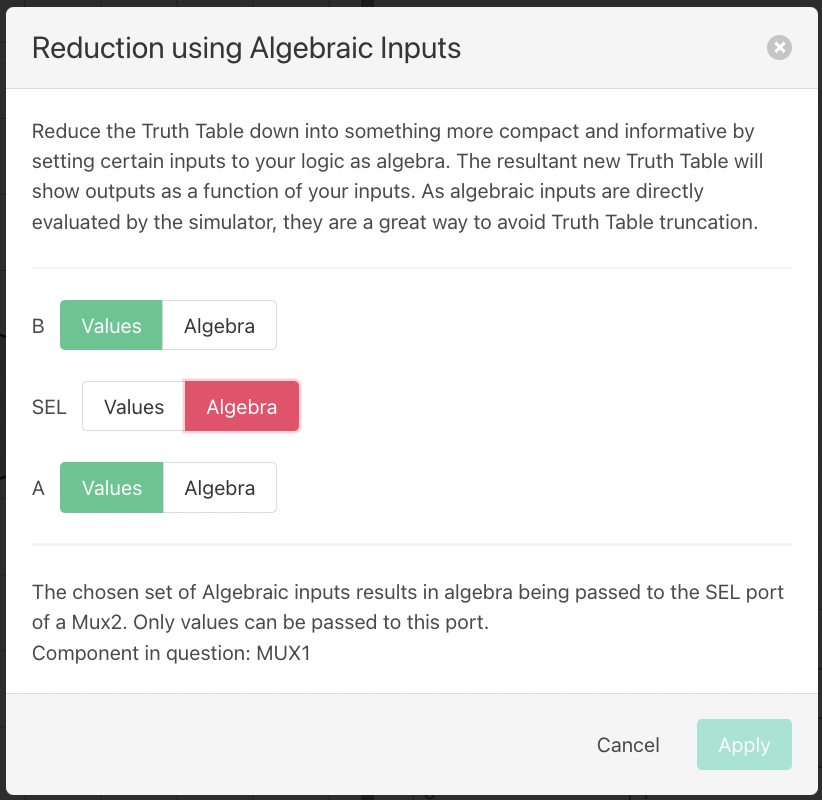
\includegraphics[width=0.6\textwidth]{04.AnalysisDesign/algebrapopup.png}
    \caption{Algebra Input Selector popup}
    \label{fig:algpopup}
\end{figure}

\subsection{Designing the System for Algebra}
The design of the system for the generation of Algebraic Truth Tables was one of the most complex activities undertaken by the project, with numerous decisions being taken regarding which features to implement and the overall approach to take. The requirements stated that support for circuits containing combinations of multiplexers and adders was the bare minimum (\textbf{D1.1.1}), but ideally Issie should support algebra for most combinational circuits.

\subsubsection{Decision 1: Algebraic Reduction vs Algebraic Generation}
It was originally envisaged that algebraic truth tables would be obtained through reduction. An exhaustive numeric truth table would be generated, and algebraic relationships would be inferred from it. This could possibly have been achieved through converting the truth table into SOP form, and then reducing the resultant Boolean equation using algebraic identities or existing logic minimisation tools like Espresso. However, following some analysis of this approach, it was deemed unfit. The requirement for an exhaustive truth table limits algebraic reduction to small circuits, while the nature of multi-bit inputs in Issie makes existing  minimisation techniques difficult to integrate into the application. Therefore, it was deemed that reducing a numeric truth table to create an algebraic truth table was not a viable strategy. his meant that algebraic truth tables would have to be generated directly from the schematic.

\subsubsection{Decision 2: Schematic Analysis vs Schematic Simulation}
Following the conclusion that algebraic truth tables would have to be directly generated from the schematic, two approaches for doing so were considered. The first was to analyse the schematic and attempt to match it to a specific case (e.g. a multiplexer circuit). The idea was that each case would describe a pre-defined algebraic relationship, which would then be returned to the user. It was thought that the approach could be extended to more complex circuits by recursively searching for cases contained within the circuit. 
The second approach was far more general; introduce a method for simulating a sheet in Issie with algebraic inputs and outputs. This would be implemented as an extension to the Fast Simulator.

The advantage of the first approach was that Requirement \textbf{D1.1.1} would be fulfilled quite easily. Following the experience of writing the Canvas Correction algorithm, it was known that checking for specific cases in the canvas state was possible, and therefore recognition of multiplexer and adder circuits could be implemented quickly. However, extending it further than that could be more challenging; the canvas state is closely related to how the user has built the schematic, and there are many different ways of implementing the same logical function. Therefore, adding support for complex relationships would likely require many cases to be checked. Furthermore, repeatedly checking the canvas state for increasingly complicated cases would increase the generation time. On the other hand, adding algebra to the Fast Simulator would be a lengthy process, increasing the amount of time required to complete \textbf{D1.1.1}. However, as the Fast Simulator is already compatible with all correct Issie schematics, it would be easier to extend algebraic simulation, as required by \textbf{D1.1.2}. Merely modifying the Fast Simulator would also introduce fewer lines of code into the Issie codebase, making further maintenance easier. Additionally, adding algebraic simulation to the Fast Simulator would mean that the Step Simulator, in theory, would also be able to support algebra. 

With all points considered, algebraic simulation was chosen over analysing the schematic. The Fast Simulator has been augmented so that it can receive both numeric and algebraic values as inputs to a simulation. It will then return outputs as functions of the algebraic inputs.


\section{Considering Logic Input with Truth Tables}
In addition to visualising combinational logic, the possibility of using truth tables as a method for combinational logic input was also considered. Issie in its current form only allows for combinational logic input via the canvas; components and connections are manually arranged by the user into a valid schematic. 
The goal of the digital electronics and computer architecture curriculum at Imperial College is to first build up students’ understanding of digital circuit design using schematics, and then eventually transition to the use of Hardware Description Languages (HDLs) in subsequent modules. Component-level schematics tend to focus on the propagation of digital signals through multiple components, while HDLs describe circuits at a behavioural level, focusing on the relationships between inputs and outputs. Defining logic using truth tables could possibly bridge the learning gap between these two concepts; prompting users to shift their design approach towards the more abstracted view of functionally mapping inputs to outputs, while also providing a familiar environment (truth tables instead of Verilog) for defining those functions.

The following system was envisaged: users would be able to define a custom hierarchical component by defining the truth table for that component. This process would begin by the user providing the names and widths of each input and output on the custom component. Using the provided inputs, the input space (left hand side) for the component's truth table would be calculated and displayed to the user with a blank right hand side. For small input spaces, the user could manually enter the output corresponding to each input row. For larger input spaces, the user would be prompted to set certain inputs as algebra, and populate the outputs with algebraic expressions which were a function of the inputs. The arguments for and against implementing this system were considered, and are presented in Table \ref{tab:logicinput}. While there was a concern that giving users a way to directly define components may detract from them learning schematic design, it was decided that from an educational perspective the system would improve Issie. However, certain issues with the implementation of algebraic truth tables for logic input were identified. A GUI would have to be developed for users to enter algebraic expressions; these would then have to be lexed and parsed. This activity was estimated to take a significant amount of time. Additionally, the algebraic relationships would have to be converted to Verilog. It was deemed that the educational benefit brought by implementing logic creation through user-entered truth truth tables was outweighed by the time investment necessary to implement the system, and that more tangible returns could be achieved by focusing that time elsewhere.

\begin{table}[!ht]
    \centering
    \begin{tabular}{|m{7cm}|m{7cm}|}
    \hline
        Pros & Cons \\ \hline
        Can help bridge the conceptual gap between component-level design and more abstracted HDL design patterns. & While gate-level design and HDLs are widely used in industry, Issie's algebraic truth table system is not standard. Therefore, using it may not transfer well into later education or industry. \\ \hline
        Would decrease the time spent designing specific components, as specific gate level operations need not be considered. This improves the user experience. & Decreasing the number of times students build gate-level designs could itself detract from their learning experience. \\ \hline
        Flexible, users can choose to define all cases or use algebraic expressions to define the component. For example, inputs which control certain parameters of operation can be left as numeric values, while operands to functions can be defined as algebraic expressions. & A GUI for entering truth tables will have to be created. Additionally, to support algebra a GUI, as well as a lexer and syntax checker will have to be created -- this is will take a significant amount of time. If algebra is not implemented, truth table definitions may only be used to define less complex components, decreasing the effectiveness of the system. \\ \hline
        ~ & Issie schematics currently can be exported as Verilog. Therefore, a function for converting a truth table component to Verilog would have to be written. This is straightforward for pure numeric truth tables, but challenging for algebraic truth tables. \\ \hline
    \end{tabular}
    \caption{Arguments for and against implementing truth-table defined custom components}
    \label{tab:logicinput}
\end{table}



% \subsection{Generating Numeric Truth Tables}
% The primary aim of the project was the generation of truth tables with interactive features to aid in logic visualisation. Thus truth table generation lies at the is a key part of the application logic. When the user first generates a truth table by clicking on the \textit{Generate Truth Table} button, a numerical truth table is generated and shown to them.
% At its core, generating a complete numeric truth table is a brute-force process. Each possible combination of input values must be simulated to calculate the corresponding output values, and the relationship should be recorded in the table. 
% Given that Issie already features a performant and reliable simulator (step simulator) for calculating the outputs of combinational logic, the decision was made to use as much of its implementation as possible. This approach has many advantages:
% \begin{itemize}
%     \item The existing step simulator has been extensively tested by end-users, meaning that its implementation is most likely bug-free. By using it, it will reduce the chance of the new feature introducing new bugs.
%     \item In most cases, reusing existing code is much faster than writing new code from scratch. Not only is time saved on writing new code, but the amount of time spent debugging is also reduced.
%     \item Reusing existing code will help keep the overall size of the codebase small. Not only does this help future programmers who work on the project by reducing how much they have to understand, but it also means that any future improvements made to the simulation code are also improvements to Truth Table generation.
% \end{itemize}

% Figure \ref{fig:flowchartSim} provides an overview of Issie's process for building and running a Step Simulation. In this process, various checks must be performed; firstly the logic designed by the user must be verified to be syntactically correct, secondly the organisation of project files must be correct, and thirdly some Issie specific limitations (e.g. no cycles in combinational logic) must be enforced. Issie's simulation building process can be said to have three levels, with each level having an associated data structure which represents schematic. These data structures are: the \textbf{Canvas State}, \textbf{Simulation Data/Error}, and a \textbf{Fast Simulation}. A set of checks are performed at each level, and only upon passing these checks can a schematic be transformed to the subsequent data structure.
% If any of these checks fail due to an issue with the user's schematic, the simulation building process returns a \textit{SimulationError}, which tells the user what the error is and which components/connections are affected. A key takeaway from Figure \ref{fig:flowchartSim} is that the process of building a simulation is separate to the process of running it. During the \codestyle{FastSimulation} building process, the schematic is analysed, with components being placed into an appropriate order for combinational reduction. However, as the \codestyle{FastSimulation} data structure is mutable, the values of each input can be updated without having to rebuild the whole simulation. Therefore, the time taken simulating a different input combination is quite short, as only the reduction function has to be re-run to find the new outputs. 
% This distinction between building a simulation and running it with different input values makes the existing Step Simulator an optimal choice for use in truth table generation, which will need to simulate multiple input combinations as fast as possible. 

% \begin{figure}
%     \centering
%     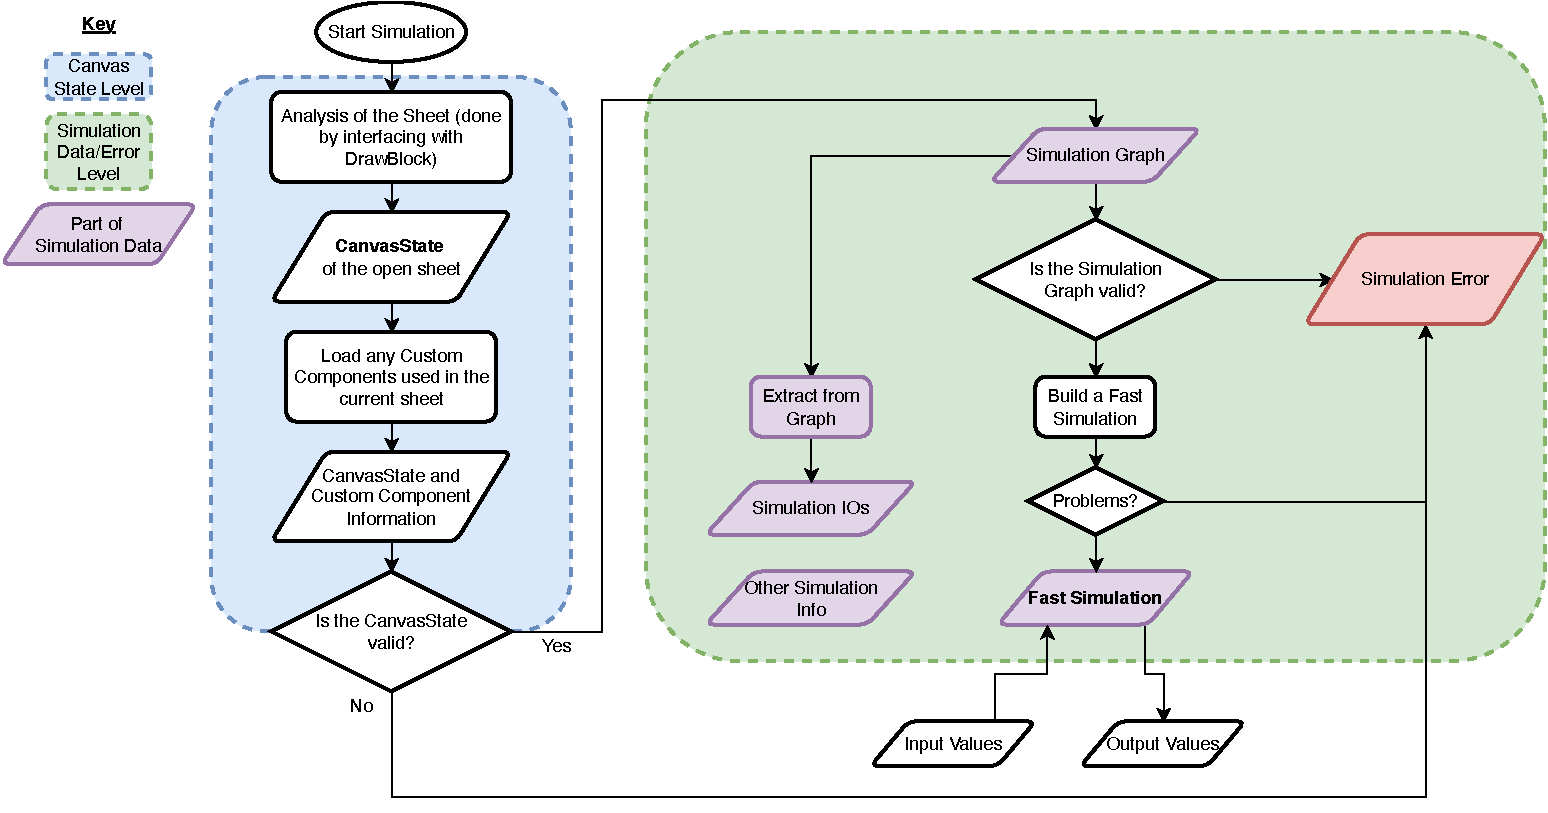
\includegraphics[width=\textwidth]{04.AnalysisDesign/IssieSim.pdf}
%     \caption{An overview of Issie's Step Simulation}
%     \label{fig:flowchartSim}
% \end{figure}

% Figure \ref{fig:ttGen} shows a high-level view of truth table generation in Issie. A simulation for the sheet is built using data stored in the current application state -- when generating truth tables for the whole sheet, this process is the same as the one which happens when starting the Step Simulator. When generating a truth table for a partial selection of a sheet, a few extra steps are required prior to the simulation building logic being called. The Step Simulator informs users of the correctness of their schematic through colour coded buttons. If the schematic is correct, the user will be shown a green button which allows them to start a simulation. On the other hand, if there are mistakes in the schematic, the user will instead be shown the \textit{See Problems} button, which will explain the nature of the Simulation Error. This functionality is replicated for the truth table, as it clearly informs the user of errors in their schematic. An additional check is also implemented for truth tables; the schematic must \textbf{only contain combinational logic}.

% If the checks for correctness and combinational logic pass, truth table generation can proceed. Alongside the Simulation Data, the truth table generation logic also requires information such as the input constraints and which inputs are algebraic. In Issie, truth tables are initially generated without any constraints or algebraic inputs, and are re-generated when these are added. Therefore, when the user clicks the button, these parameters are empty. From this information, the input space of the truth table (its left-hand side) is determined. Each input combination is then simulated, with the output and viewer values corresponding to that combination recorded and stored. A truth table is simply the mapping between input and output combinations - this mapping is stored so that it may later be viewed in tabular form by the View function.

% \begin{figure}[h]
%     \centering
%     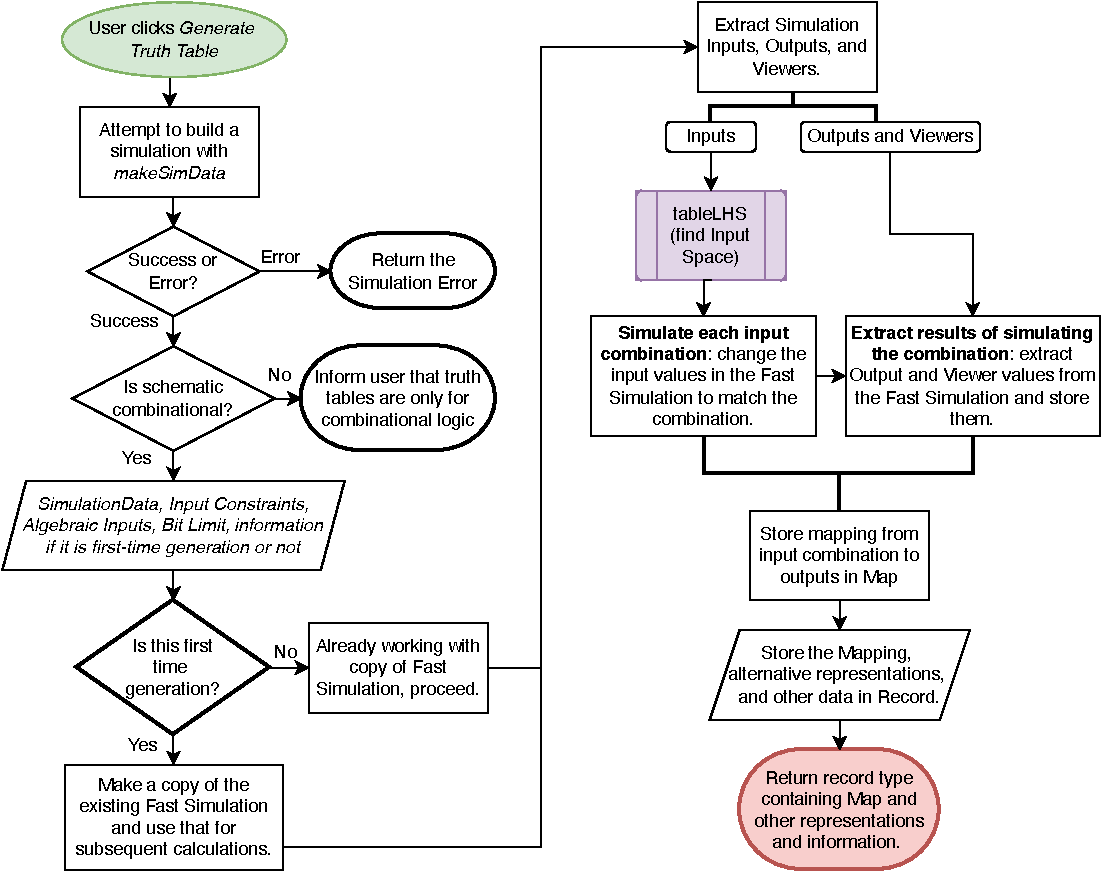
\includegraphics[width=\textwidth]{04.AnalysisDesign/ttGen.pdf}
%     \caption{High-Level view of Truth Table Generation}
%     \label{fig:ttGen}
% \end{figure}

% The process of calculating the input space, highlighted in purple in Figure \ref{fig:ttGen} had two versions; the change from the first to the second affected the overall structuring of operations on truth tables in the application. Initially, the entire input space was calculated and simulated. This would result in a very large, exhaustive truth table -- one which contained every possible input and output combination. The user would haven been able to reduce this truth table by filtering the table or using Don't Care Reduction. However, several issues arose with this approach, with the most crucial being that of performance. The complexity of finding the Cartesian product of multiple sets is an exponential function of the number of sets. For example, the complexity of finding the Cartesian product of $n$ sets, each of size $s$, would be $O(s^n)$. The size of each set is dependent on the width of the input; Issie does not limit input widths, meaning that the size of the sets may also be very large. For example, a single 16-bit input has 65536 unique values, and combining this with a second 16-bit input yields an input space of over 4 billion unique combinations. Simulating this large number of combinations and storing the result takes upwards of 20 seconds, violating essential requirement \textbf{E1.7}. Additionally, a sufficiently large input space could cause the system to run out of memory and crash, which is totally unacceptable. Along with the practical issues with the generation of the complete truth table, it can also be argued that a very large complete truth table is not useful to the user. According to the Atkinson-Shiffrin memory model described in Section \ref{subsec:memmodels}, external stimuli only stay in the sensory register for 0.5 seconds prior to decaying. A large number of rows is likely to overload the sensory register, meaning that it is likely that the information will not pass to short term memory unless the the user slows down and processes each row one-by-one. Even if this were the case, a truth table with a large number of rows would take over 30 seconds for the user to read and process. Given that short term memory decays in 30 seconds, this means that the user will likely have forgotten the first row by the time they finish reading the last one. Therefore, the method of generating and simulating the entire input space to create an exhaustive truth table was deemed unfit.

% As a result, the decision was made to \textbf{truncate the truth table}; generate and simulate only part of the input space. The current limit is 1024 rows. Considering that users would only be able to focus on a small subset of rows at a time, and would likely reduce the size of the table anyways, this approach would sacrifice very little for a significant gain. However, any subsequent operations, such as filtering and reduction, would take place on the truncated table, which does not contain all of the necessary data. The nature of these issues, as well as the steps taken to mitigate them are:

% \begin{itemize}
%     \item[] \textbf{Issue 1}: Input constraints will be applied to the truncated table, so user may not see a full representation of the relationships for the case they enter. For example, consider the input $X$ which has a width of 8 bits (so values range from 0 to 255), but due to truncation, only rows with values of $X$ up to 31 are present. If the user applies the input constraint $X = 32$ to the table, an empty table will be returned as no rows which fulfil this condition exist in the truncated table.
%     \item[] \textbf{Solution 1}: Apply input constraints during truth table generation. This is achieved by using the constraints to determine a tighter input space, and then simulating that. Giving users a way to choose which inputs contribute more to the input space (they can fix certain inputs and let others vary within bounds) allows them to interactively generate truth tables that deliver the most information to them.
%     \item [] \textbf{Issue 2}: Output constraints will be applied to the truncated table, which is missing many rows. Due to this, the result of applying the output constraints will include all rows which match the condition.
%     \item [] \textbf{Solution 2}: Unfortunately there is not much that can be done to combat this issue alone other than warn the user that they are looking at incomplete results. However, if the user is able to use input constraints to sufficiently reduce the input space first, output constraints could help filter the table further.
%     \item [] \textbf{Issue 3}: Don't Care Reduction will occur on the truncated table, which does not fully represent the logical function performed by the circuit. This could result in incorrect relationships being inferred by the reduction algorithm.
%     \item [] \textbf{Solution 3} Much like with output constraints, there is no perfect solution as relationships for reduction are inferred from the truth table. Don't Care reduction is therefore limited to smaller schematics which do not produce truncated truth tables. The user is instead guided towards reducing truth tables for larger schematics with \textbf{Algebraic Reduction}.
% \end{itemize}

% Implementing Solution 1 required a new method of generating the input space; a general view of the method used is shown in Figure \ref{fig:tableLHS}. As generating input combinations is expensive in terms of time and memory, the input space generation method needs to know which sub-sets of the input space it can and cannot generate before it actually generates it using the Cartesian product method. Further details of how this is implemented can be found in the Implementation chapter, with elaboration on the complex \codestyle{inputsWithARC} function (highlighted purple on Figure \ref{fig:tableLHS}).
% \begin{figure}
%     \centering
%     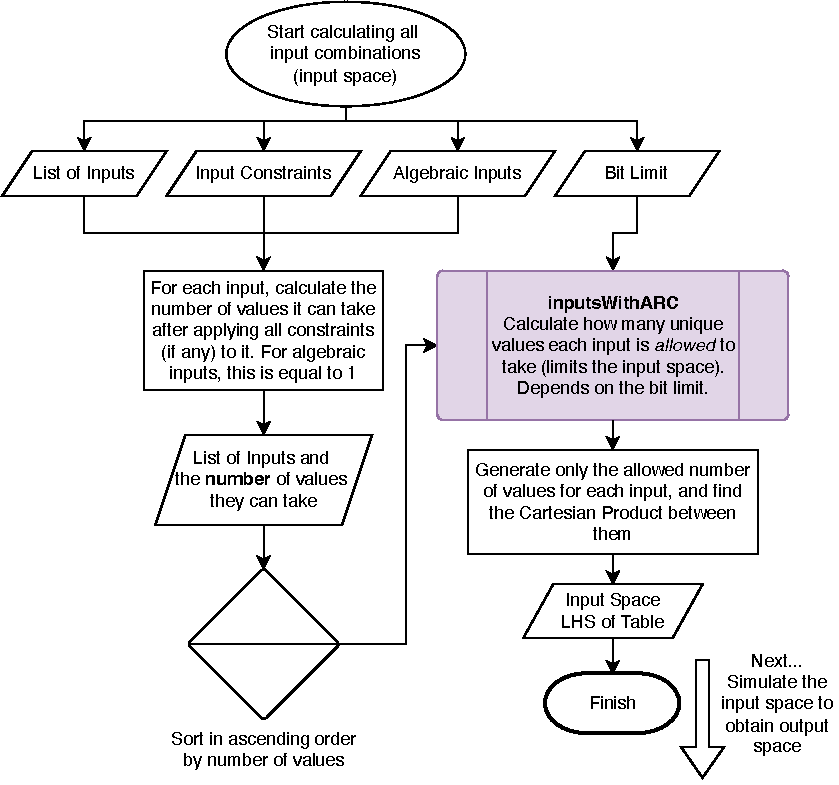
\includegraphics{04.AnalysisDesign/newLHS.pdf}
%     \caption{High-Level view of how the Input Space is generated}
%     \label{fig:tableLHS}
% \end{figure}